\section{Don Tammeo}\label{don-tammeo}

Tags: PC Alias: The Rencil Creatore: Davide Giocatore: Davide
Ispirazione: Don Matteo, Terence Hill Luogo: Eldrid Razza: Umano Classe:
Chierico Livello: 12

\section{Don Tammeo}\label{don-tammeo-1}

\begin{center}\rule{0.5\linewidth}{0.5pt}\end{center}

\begin{figure}
\centering
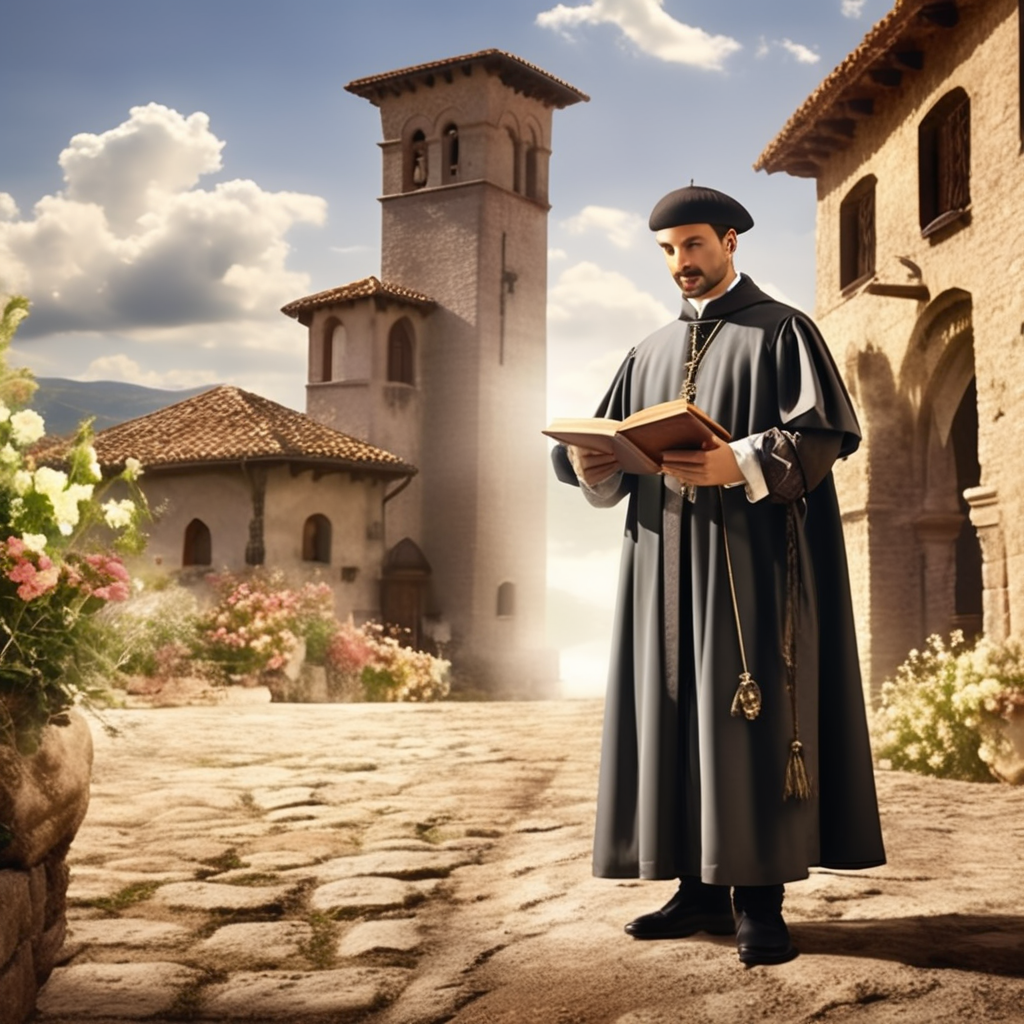
\includegraphics{create-images-of-don-matteo-the-italian-tv-character-in-a-medieval-setting-envision-him-as-a-bene.png}
\caption{create-images-of-don-matteo-the-italian-tv-character-in-a-medieval-setting-envision-him-as-a-bene.png}
\end{figure}

Informazioni Generali

Età:

Data di nascita:

Luogo di nascita: Eldrid

Razza: Umano

Classe: Chierico

Alleati:

Nemesi:

Alias:

Professione: Prete, Protettore

\begin{center}\rule{0.5\linewidth}{0.5pt}\end{center}

\subsection{1. Descrizione Generale}\label{descrizione-generale}

\begin{center}\rule{0.5\linewidth}{0.5pt}\end{center}

\begin{figure}
\centering

\includegraphics{full-body-portrait-of-a-beautiful-female-elf-with-long-silver-hairs-and-deep-green-eyes-fantasy-se-.png}
\caption{full-body-portrait-of-a-beautiful-female-elf-with-long-silver-hairs-and-deep-green-eyes-fantasy-se-.png}
\end{figure}

Don Tammeo è l'incarnazione della speranza nelle strade di Eldrid, un
orfano che ha abbracciato la fede di Luminara Libertas. Membro devoto
della Gilda dei Protettori, la sua presenza irradia compassione e
giustizia, offrendo luce in un mondo avvolto dall'oscurità.

\begin{quote}
``Tutti quanti abbiamo un estremo bisogno di sentirci amati. Ma non c'è
nessuna persona che può colmare questo infinito bisogno d'amore che
abbiamo!'' - Don Tammeo
\end{quote}

\subsection{2. Biografia}\label{biografia}

\begin{center}\rule{0.5\linewidth}{0.5pt}\end{center}

\subsubsection{\texorpdfstring{2.1
\textbf{Infanzia}}{2.1 Infanzia}}\label{infanzia}

\begin{center}\rule{0.5\linewidth}{0.5pt}\end{center}

Don Tammeo è nato sotto il cielo di
\href{Eldrid\%20bd820bb9f6164b39ae6e611a94748518.md}{Eldrid} , ma il
destino gli riservò un percorso diverso. Abbandonato alla sua sorte fin
dalla nascita, Tammeo fu accolto nelle braccia di un orfanotrofio della
città. Crescendo tra i compagni orfani, sviluppò una forza interiore
alimentata dalla necessità di sopravvivere in un mondo spietato.
Tuttavia, durante la sua infanzia, un misterioso evento cambierà il
corso della sua vita. Una notte, mentre osservava il cielo stellato da
una finestra dell'orfanotrofio, ebbe una visione rivelatrice che lo
avvicinò alla fede. Un senso di libertà pervase il suo cuore,
spingendolo a cercare il significato più profondo della vita.

\subsubsection{\texorpdfstring{2.2
\textbf{Adolescenza}}{2.2 Adolescenza}}\label{adolescenza}

\begin{center}\rule{0.5\linewidth}{0.5pt}\end{center}

Il richiamo della fede non abbandonò Don Tammeo nemmeno
nell'adolescenza. Spinto dalla visione misteriosa della sua infanzia, si
dedicò agli studi religiosi presso i templi di Eldrid. Con passione e
determinazione, prese i voti e divenne un servo devoto di una divinità
legata al culto della libertà. La sua fede non era solo un insieme di
dogmi, ma una forza guida che plasmò il suo carattere. Tammeo imparò a
condividere il messaggio di speranza e libertà con coloro che
incontrava, diventando una figura di ispirazione per gli altri giovani
che cercavano un significato nella loro esistenza.

\subsubsection{\texorpdfstring{2.3 \textbf{Età
Adulta}}{2.3 Età Adulta}}\label{etuxe0-adulta}

\begin{center}\rule{0.5\linewidth}{0.5pt}\end{center}

Don Tammeo, ora un uomo maturo con il cuore pervaso dalla fede, decise
che la sua missione doveva estendersi oltre le mura del tempio. Sentendo
il richiamo di aiutare coloro che erano in difficoltà, si unì alla Gilda
dei Protettori, un gruppo di individui devoti alla protezione e al
soccorso dei più deboli e bisognosi. La sua dedizione alla giustizia e
la sua connessione con la divinità lo resero un membro rispettato della
gilda. Armato della sua fede incrollabile e della sua compassione per
gli altri, Don Tammeo si adoperò per risolvere i crimini, difendere gli
indifesi e portare la luce della libertà in ogni angolo oscuro di
Eldrid. La sua storia, da orfano a protettore, è diventata una fonte di
ispirazione per la comunità che ha giurato di servire.

\subsection{3. Carriera}\label{carriera}

\begin{center}\rule{0.5\linewidth}{0.5pt}\end{center}

Dopo aver preso i voti e aver dedicato la sua vita alla fede di Luminara
Libertas, Don Tammeo ha iniziato il suo cammino come sacerdote
itinerante. Ha viaggiato per Eldrid e le terre circostanti, portando il
messaggio di libertà, speranza e giustizia alle persone che incontrava.
La sua fama di uomo di fede e protettore dei bisognosi ha attirato
l'attenzione della Gilda dei Protettori.

La Gilda, riconoscendo la saggezza e la dedizione di Don Tammeo, lo ha
invitato ad unirsi a loro. Egli ha accettato l'invito, portando la sua
prospettiva unica e il suo zelo per la giustizia all'interno della
gilda. La sua carriera nella Gilda dei Protettori è caratterizzata da
numerosi successi nell'aiutare coloro che sono vittime di ingiustizia e
nell'affrontare minacce criminali.

Don Tammeo ha guadagnato il rispetto dei suoi compagni di gilda e della
comunità di Eldrid, diventando un leader spirituale oltre che un
protettore fisico.

\subsection{4. Personalità}\label{personalituxe0}

\begin{center}\rule{0.5\linewidth}{0.5pt}\end{center}

Don Tammeo è un'anima gentile, permeata da una compassione inesauribile.
La sua gentilezza si manifesta attraverso ogni parola e azione, offrendo
conforto a chi è in difficoltà e speranza a coloro che ne hanno bisogno.
La sua fede profonda, ancorata al culto di Luminara Libertas, si traduce
in una determinazione instancabile nel perseguire la libertà e la
giustizia per tutti. Tammeo incarna l'ottimismo, vedendo la luce della
speranza anche nei momenti più bui. La sua integrità morale è come una
guida luminosa, ispirando gli altri a seguire un cammino di rettitudine.
In seno alla Gilda dei Protettori, Don Tammeo assume il ruolo di leader
spirituale, le sue parole fungono da faro guida e il suo impegno per la
causa della libertà crea un legame indissolubile con coloro che
condividono la sua missione. La sua presenza, carica di saggezza e
amore, si staglia come un rifugio sicuro per chi cerca giustizia e
speranza nelle terre di Eldrid

\subsection{A. Coinvolgimenti in Eventi
Recenti}\label{a.-coinvolgimenti-in-eventi-recenti}

\begin{center}\rule{0.5\linewidth}{0.5pt}\end{center}

\href{Untitled\%20Database\%204072dbc4c66843f698664cd6770495dc.csv}{Untitled
Database}

\subsection{B. Aggiornamenti}\label{b.-aggiornamenti}

\begin{center}\rule{0.5\linewidth}{0.5pt}\end{center}

\href{Untitled\%20232ee623461a495b99cb6e5142aa9435.csv}{}

\subsection{C. Galleria Immagini}\label{c.-galleria-immagini}
